\section{PAIRED UNCERTAINTY OVER THE COMPLETE DOSE GRID}
For each training seed, subtract random-removal FDP (or power) from the corresponding exposure-removal value after averaging its five test splits and fifty calibration repetitions. Report the mean of ten paired differences and the pointwise interval $\bar d\pm t_{9,.975}s_d/\sqrt{10}$. This estimates repeated-training/evaluation uncertainty on the given graph, not variation across graphs. The intervals are pointwise and do not adjust for searching across conditions. The complete grid is shown rather than retaining only positive intervals.
\begin{figure*}[t]\centering
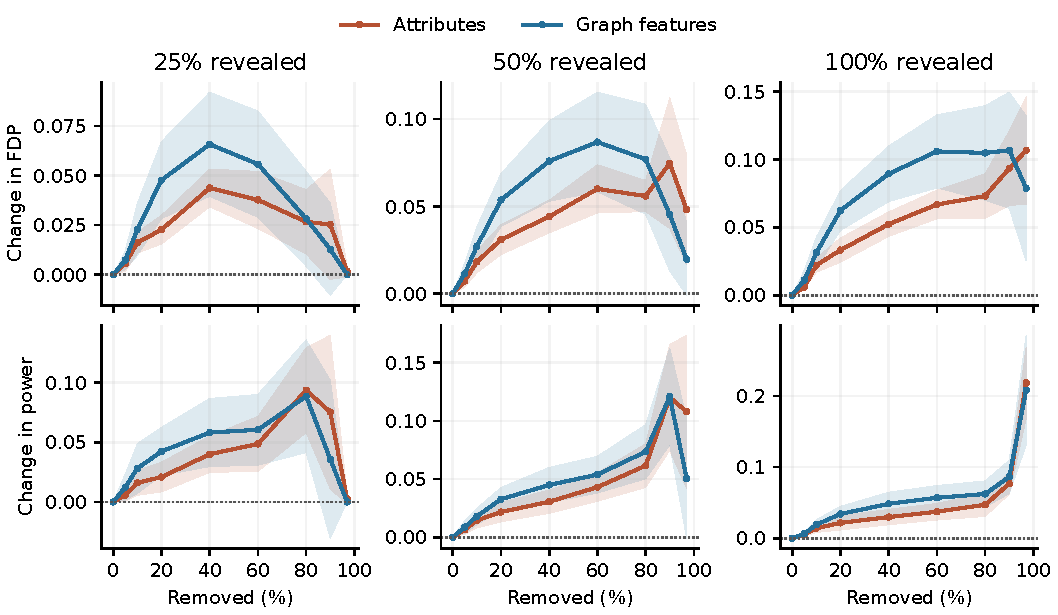
\includegraphics[width=\textwidth]{dose_paired_amazon.pdf}
\caption{Amazon: exposure removal minus size-matched random removal over the complete dose grid. Shading gives pointwise 95\% paired $t$ intervals across ten training-seed averages after averaging splits and calibration repetitions. Intervals describe repeated evaluation conditional on this graph; they are neither simultaneous across the sweep nor uncertainty over new graphs.}
\end{figure*}

\begin{figure*}[t]\centering
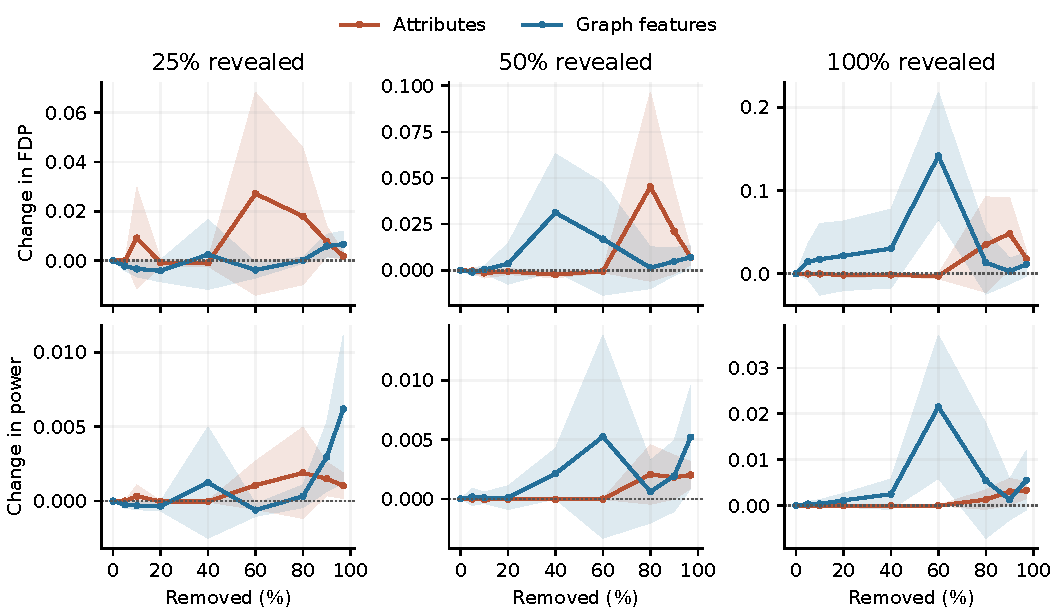
\includegraphics[width=\textwidth]{dose_paired_tolokers.pdf}
\caption{Tolokers: exposure removal minus size-matched random removal over the complete dose grid. Shading gives pointwise 95\% paired $t$ intervals across ten training-seed averages after averaging splits and calibration repetitions. Intervals describe repeated evaluation conditional on this graph; they are neither simultaneous across the sweep nor uncertainty over new graphs.}
\end{figure*}

\begin{figure*}[t]\centering
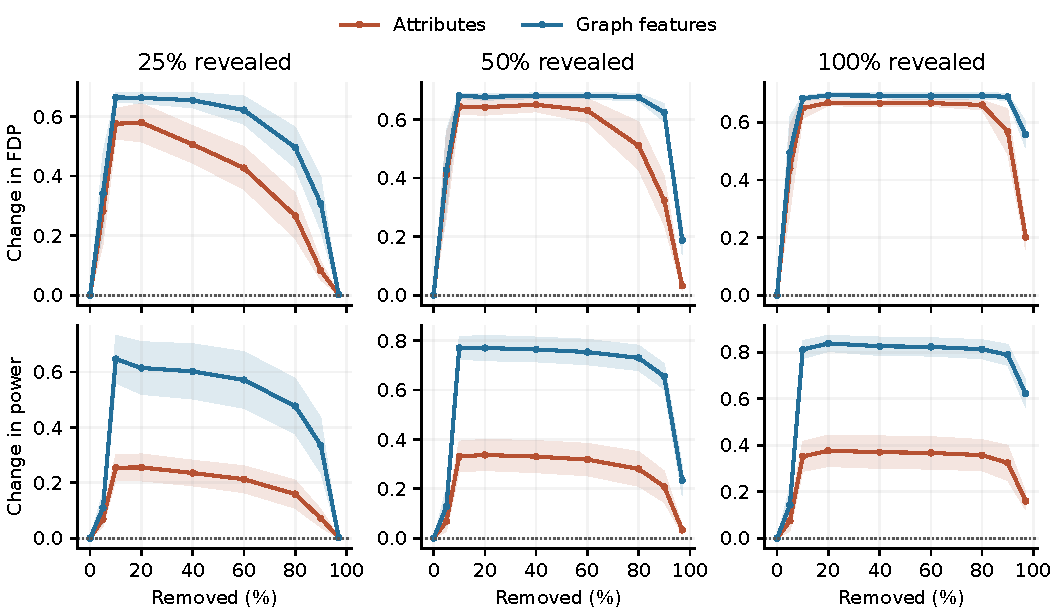
\includegraphics[width=\textwidth]{dose_paired_weibo.pdf}
\caption{Weibo (PyGOD): exposure removal minus size-matched random removal over the complete dose grid. Shading gives pointwise 95\% paired $t$ intervals across ten training-seed averages after averaging splits and calibration repetitions. Intervals describe repeated evaluation conditional on this graph; they are neither simultaneous across the sweep nor uncertainty over new graphs.}
\end{figure*}

\begin{figure*}[t]\centering
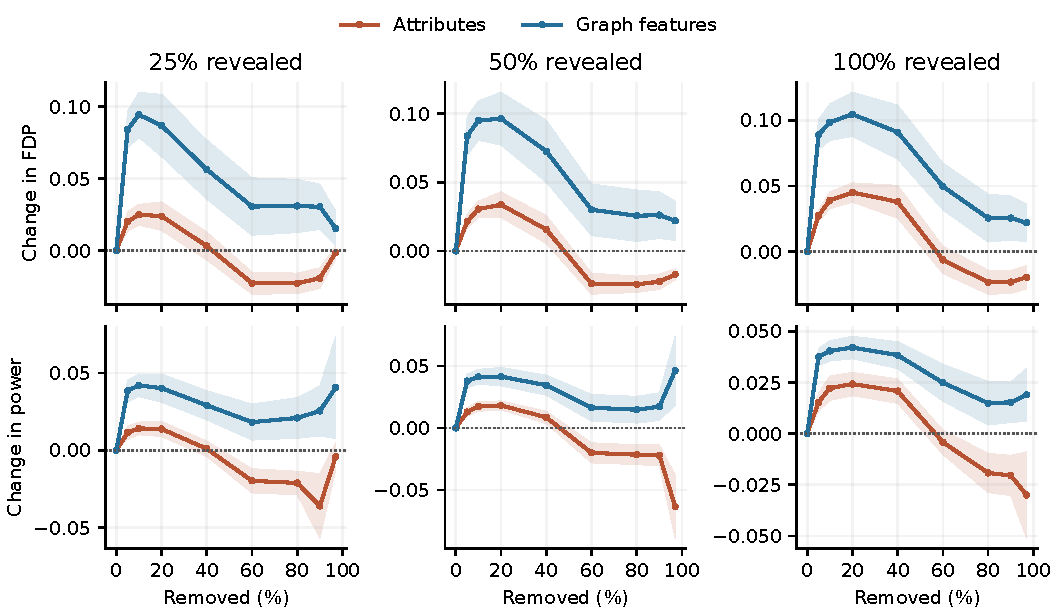
\includegraphics[width=\textwidth]{dose_paired_tfinance.pdf}
\caption{T-Finance: exposure removal minus size-matched random removal over the complete dose grid. Shading gives pointwise 95\% paired $t$ intervals across ten training-seed averages after averaging splits and calibration repetitions. Intervals describe repeated evaluation conditional on this graph; they are neither simultaneous across the sweep nor uncertainty over new graphs.}
\end{figure*}

\begin{figure*}[t]\centering
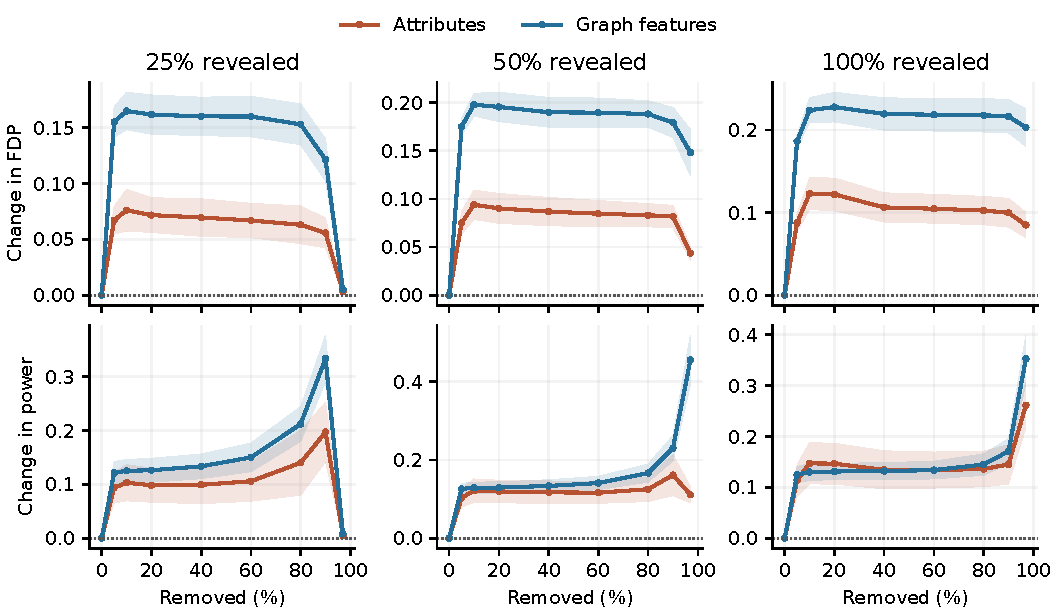
\includegraphics[width=\textwidth]{dose_paired_weibo_gadbench.pdf}
\caption{Weibo (GADBench): exposure removal minus size-matched random removal over the complete dose grid. Shading gives pointwise 95\% paired $t$ intervals across ten training-seed averages after averaging splits and calibration repetitions. Intervals describe repeated evaluation conditional on this graph; they are neither simultaneous across the sweep nor uncertainty over new graphs.}
\end{figure*}